\documentclass[a4paper, 10pt]{article}
\usepackage[utf8x]{inputenc}
\usepackage{graphicx}
\usepackage{geometry}
\usepackage{amsmath}
\usepackage{mathenv}
\usepackage{amssymb}
\usepackage{amsfonts}
\usepackage{mathrsfs}
\usepackage{textcomp}
\geometry{hmargin = 2.5cm, vmargin = 1.5cm}

% OPENING
\title{SY09 - TP04\\Analyses discriminantes quadratique et linéaire}
\author{Bertrand Bon - Antoine Hars}

\begin{document}

\maketitle

\section*{Introduction}
Dans le cadre de ce tp, nous avons étudié les analyses discriminantes quadratique et linéaire.\\ \\

\section*{Exercice 1 : Règle de Bayes.}
On suppose que la population est répartie en deux classes, en proportions $\pi_{1}$ et $\pi_{2}$ = 1 - $\pi_{1}$,
issues des distributions gaussiennes bivariées $\mathcal{N}(\mu_{1}, \Sigma_{1})$ et $\mathcal{N}(\mu_{1}, \Sigma_{1})$.\\

\subsection*{1. Donner une équation de la frontière de décision de la règle de Bayes dans chacun des cas suivants :}

\subsubsection*{(a) $\pi_{1}$ = 0.5, $\mu_{1}$ = (0,0)´, $\mu_{2}$ = (1,1)´, $\Sigma_{1}$ = $\Sigma_{2}$ =
$\begin{pmatrix} 1 & 0 \\ 0 & 1 \end{pmatrix}$ :}
% TODO

\subsubsection*{(b) $\pi_{1}$ = 0.1, $\mu_{1}$ = (0,0)´, $\mu_{2}$ = (1,1)´, $\Sigma_{1}$ = $\Sigma_{2}$ =
$\begin{pmatrix} 1 & 0 \\ 0 & 1 \end{pmatrix}$ :}
% TODO

\subsubsection*{(c) $\pi_{1}$ = 0.5, $\mu_{1}$ = (0,0)´, $\mu_{2}$ = (1,1)´, $\Sigma_{1}$ = $\Sigma_{2}$ =
$\begin{pmatrix} 1 & -0.3 \\ -0.3 & 1 \end{pmatrix}$ :}
% TODO

\subsubsection*{(d) $\pi_{1}$ = 0.6, $\mu_{1}$ = $\mu_{2}$ = (1,1)´, $\Sigma_{1}$ = $\begin{pmatrix} 1 & 0 \\ 0 & 1 \end{pmatrix}$,
$\Sigma_{2}$ =  $\begin{pmatrix} 5 & 0 \\ 0 & 5 \end{pmatrix}$ :}
% TODO

\subsubsection*{(e) $\pi_{1}$ = 0.6, $\mu_{1}$ = (0,0)´, $\mu_{2}$ = (1,1)´, $\Sigma_{1}$ = $\begin{pmatrix} 1 & 0 \\ 0 & 1 \end{pmatrix}$,
$\Sigma_{2}$ = $\begin{pmatrix} 1 & 0.5 \\ 0.5 & 1 \end{pmatrix}$ :}
% TODO


\subsection*{2. Simulation de la règle de Bayes dans R :}
Pour chacune des cinq populations précédentes, en utilisant la fonction \textit{simul} réalisée au TD3 (Théorie de la décision),
nous avons généré un échantillon de taille \textit{n} = 1000.\\
Pour rappel, le code de la fonction \textit{simul} est comme suit :\\
\begin{verbatim}
simul <- function (n, pi, mu1, mu2, sigma1, sigma2) {

  # On crée la matrice contenant l'échantillon résultat de la fonction.
  result = matrix(nrow = n, ncol = 3)

  # Affectation de chaque élément de l'échantillon final à la classe 0 ou 1.
  for (k in 1:n) {

    rand = sample(0:1, 1)
    result[k, 3] = rand

    if (result[k, 3] == 0) {
      result[k, c(1, 2)] = mvrnorm(1, mu1, sigma1)
    } else {
      result[k, c(1, 2)] = mvrnorm(1, mu2, sigma2)
    }
  }

  return (result)
}
\end{verbatim}
$\\ \\$
Pour chacun des échantillons de population, nous avons tracé les nuages suivants associés,
avec le tracé de la frontière de décision pour les trois premiers cas :\\
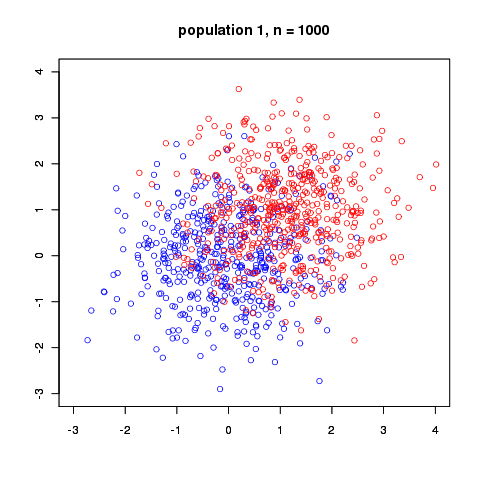
\includegraphics[height = 7cm, width = 7cm]{plots/exo1_simul_1.png}
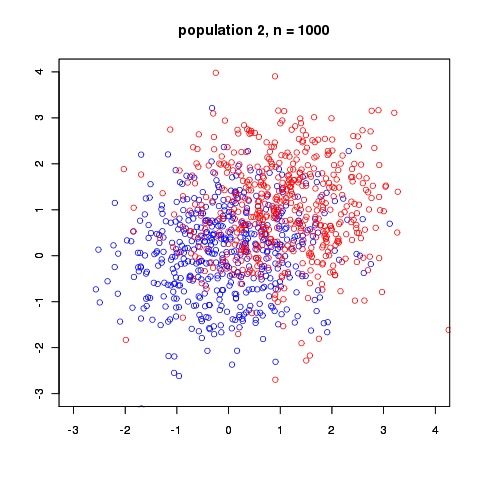
\includegraphics[height = 7cm, width = 7cm]{plots/exo1_simul_2.png}\\
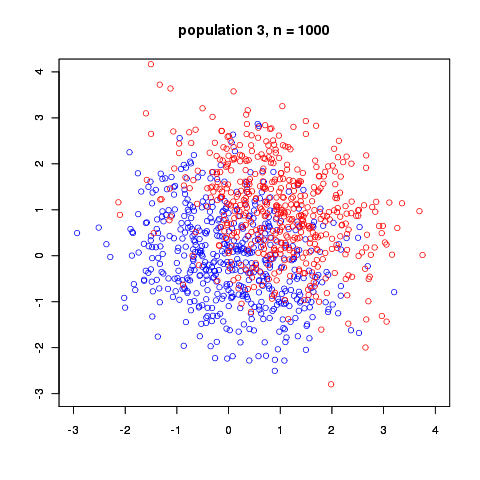
\includegraphics[height = 7cm, width = 7cm]{plots/exo1_simul_3.png}
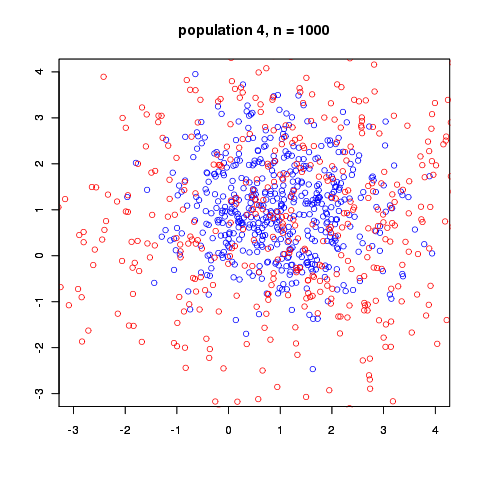
\includegraphics[height = 7cm, width = 7cm]{plots/exo1_simul_4.png}\\
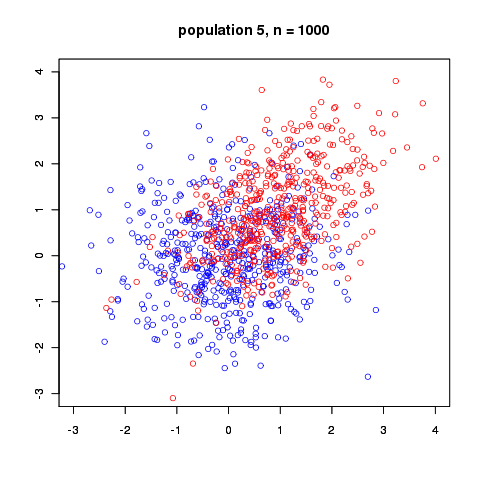
\includegraphics[height = 7cm, width = 7cm]{plots/exo1_simul_5.png}\\ \\
%TODO frontière de décision pour les 3 premiers cas.

Pour chaque cas de figure, nous avons déterminé l'expression d'un estimateur de la probabilité d'erreur,
ainsi que sa réalisation sur l'échantillon correspondant.\\
% TODO
Cela nous a permis de le comparer avec la probabilité d'erreur théorique.\\
% TODO

\section*{Exercice 2 : Analyse discriminante sur les données \textit{Crabes}.}

\subsection*{1. Expliquer en deux lignes ce que fait chacune des fonctions :}
\textbf{lda :} Cette fonction sert à effectuer l'analyse discriminante linéaire qui cherche à détecter sur la matrice de covariance est singulière.\\
Cette fonction peut être appelée avec en paramètre une formule, un data frame, une matrice.\\
\textbf{qda :} Cette fonction est utilisée pour effectuer l'analyse discriminante quadratique en utilisant une décomposition QR qui retournera un message d'erreur si la variance du groupe est singulière pour chaque groupe.\\
\textbf{contour :} Cette fonction est utile pour créer un graphe de contour ou pour ajouter une ligne de contour à un graphe existante.\\
\textbf{sample :} Cette fonction nous permet de récupérer un échantillon de taille spécifiée d'éléments de l'ensemble X.\\
\textbf{predict :} Predict() est une fonction générique de prédictions de modèle.\\
\textbf{predict.lda :} Cette fonction classifie des observations multi-variables en utilisant l'analyse discrimante linéraire.\\
\textbf{Comparaison entre predict et predict.lda :} predict est générique et predict.lda non.\\ \\
\subsection*{}
\subsection*{}
\subsection*{}

\section*{Exercice 3 : }

\subsection*{}
\subsection*{}
\subsection*{}

\section*{Conclusion}

\end{document}
